\documentclass{beamer}

\usepackage{graphicx}
\usepackage{caption}
\usepackage{subcaption} % for subfigure
\usepackage{hyperref}
\usepackage{amssymb}
\usepackage{tabularx}
\usepackage{multicol}
\usepackage{algpseudocode}
\usepackage{amsthm} % for theorem
\usepackage{algorithm}
\usetheme{Warsaw}
\title[HRA for Concurrent Programs] % (optional, only for long titles)
{Heap Analysis for Concurrent Programs}
\subtitle{BTP-2 Presentation}
\author[Anshul Purohit] % (optional, for multiple authors)
{
Anshul Purohit \\
Roll No: 110050002 \\
}
\institute[Universitäten Hier und Dort] % (optional)
{
	Indian Institute of Technology Bombay
}
\date[KPT 2004] % (optional)
{
Guide: Prof. Uday Khedker \\
}
\subject{Informatik}


\begin{document}
\frame{\titlepage}
\begin{frame}

\frametitle{Outline}
\begin{itemize}
\item Introduction to Problem Statement
\item Heap Analysis 
\item Analysis technique of Concurrent Programs
\item Problems with the technique
\item Improvements 
\end{itemize}
\end{frame}
	
  \begin{frame}
  \frametitle{Introduction}
  \begin{itemize}
  \item Designing an technique for carrying
  out heap reference analysis of concurrent programs.
  \item Reference expression like \emph{x.lptr.rptr.data} are primarily used to access the objects in the heap.
  \item Will primarily focus on determining the  liveness of access links to objects on the heap.
  \item Java model: The root variables, which are stored on stack, represent references to memory in heap.
     
  \end{itemize}
  \end{frame}
  
  \begin{frame}
  	\frametitle{Introduction}
  	
  	 Model of threads used to refer to concurrent programs in the problem.
  	\begin{itemize}
  		\item For accessing shared data,
  		critical sections need to be guarded by the lock and unlock statements.
  		\item Also, we would work under the assumption that program would be data-race free.
  		\item Will present a technique to perform analysis for concurrent programs.  
  		
  	\end{itemize}
  	
  \end{frame}
  
  \begin{frame}
\frametitle{Heap Analysis}
	Analyzing properties of heap data is not very trivial.  

\begin{itemize}
	\item The structure of stack and static data is simple to understand since stack variables have a compile-time name(alias) associated with it.
	\item However, heap data has no compile time alias associated. Also the mapping of access expressions to memory location can change during program execution.
	\item Objects are referred based on their allocation site.
\end{itemize}
  \end{frame}
  
  
  
  
% RELATED WORK %
  \begin{frame}
  \frametitle{Heap Analysis}
  %\framesubtitle{Related Work}
	Heap analysis tries to find out the answer to the questions: 
	\begin{itemize}
		\item Can an access expression $a_1$ at program point $p_1$ have the same l-value as access expression $a_2$ at program  point $p_2$.
		\item Can there exist objects in the heap that will not be reachable from the access expressions in the program?
		\item Which of the access links will be live at a particular point?
	\end{itemize}
	We will focus on the liveness analysis part of the heap reference analysis.
	\end{frame}
\begin{frame}
\frametitle{Points-to analysis for Java}
  %\framesubtitle{Related Work}
	In Java pointers are not created explicitly. All objects in Java are accessed using references. Points-to analysis for Java programs identifies the objects pointed to by references at run time.
	
	\begin{figure}[here]
	\begin{center}
	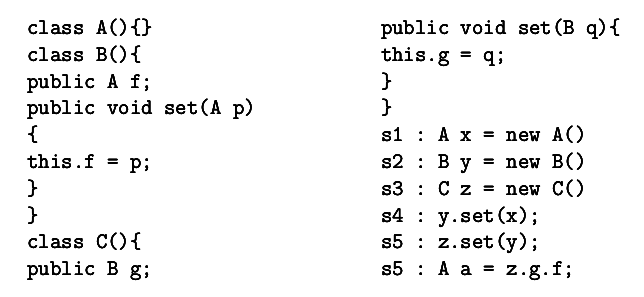
\includegraphics[width=8cm]{Figures/rsz_heap.png}
	\end{center}
	\caption{Example for heap access and points-to}
	\label{fig:ex1}
	\end{figure}
	
	
	
  \end{frame}

  \begin{frame}
  \frametitle{Points-to Graph}
  %\framesubtitle{Related Work}
	Points-to graph in Java contain two types of edges. The first type of edge is to represent the information that reference variable $v$  is pointing to object $o$. The second type of edge represents the field $f$ of $o_1$ pointing to $o_2$.

	\begin{figure}[here]
		\begin{center}
			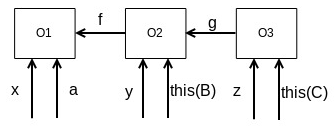
\includegraphics[width=7cm]{Figures/rsz_points_to_graph.png}
		\end{center}
		\caption{Example for points-to graph}
		\label{fig:ex1}
	\end{figure}

  \end{frame}

\begin{frame}
\frametitle{Heap Reference Analysis}

A reference can be represented by an access path. In order to perform liveness analysis of heap and identify the set of live links, naming of links is necessary.

%An Access Path is defined as root variable name following any number of field names and is represented as $x$ $\rightarrow$ $n_1$ $\rightarrow$ $n_2$ .... $\rightarrow$ $n_k$ where $x$ is root variable, $n_1$ , $n_2$ .. $n_k$ are field names.

	\begin{figure}[here]
		\begin{center}
			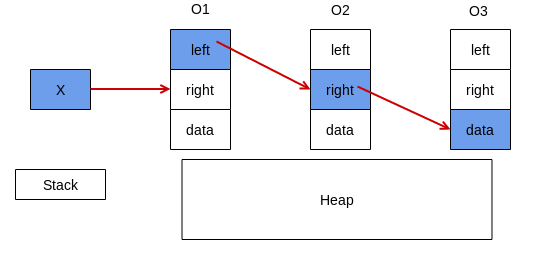
\includegraphics[width=8cm]{Figures/hra_access_path.png}
		\end{center}
		\caption{access path for the expression \emph{x.left.right.data}}
		\label{fig:accpath}
	\end{figure}

\end{frame}

\begin{frame}
\frametitle{Heap Liveness Analysis}

An access path can be unbounded in the case of loops. We need to set a bound on the representation of access paths for liveness information. This is achieved using access graphs. Summarization would also require including program points.

\begin{figure}[here]
	\begin{center}
		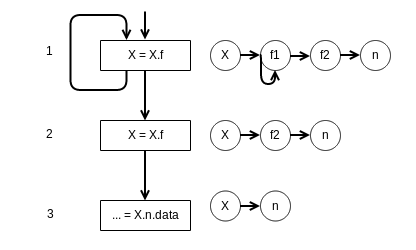
\includegraphics[width=7cm]{Figures/heap_summarization_liveness.png}
	\end{center}
	\caption{Use of access graph and liveness data flow values}
	\label{fig:accpath}
\end{figure}

\end{frame}



% RULE SETS %
  \begin{frame}
  \frametitle{Inter-procedural analysis}
  %\framesubtitle{Analysing existing rule sets}
  Inter-procedural Analysis is required to obtain more precise results as it is very common that programs can have multiple function calls.
  \begin{itemize}
	\item It is essential to consider the effect of function call on the data flow value entering the node.
	\item Inter-procedural analysis takes into account call return , parameter passing , local variables of the function, return values and recursion into account
	\item Major issue to be dealt while handling inter-procedural analysis is to deal with calling contexts.
	\item Context-Sensitive analysis
	\end{itemize}
  \end{frame}
  
  \begin{frame}
  \frametitle{Call Graph}
  %\framesubtitle{Analysing existing rule sets}
  \begin{itemize}
  	\item Static data structure representing run-time calling relationships among procedures.
  	\item Call multi-graph is a directed graph which represents calling relationships.
  	\item In Super graph callsites are connected to the callee procedure entry node and the exit node is connected to return node in the caller.
  \end{itemize}

  \end{frame}

  \begin{frame}
  \frametitle{Example}
  		\begin{figure}[here]
  			\begin{center}
  				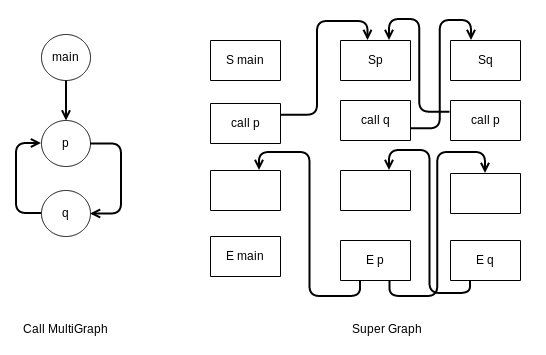
\includegraphics[width=10cm]{Figures/callgraph.png}
  			\end{center}
  			\caption{Call Multi-graph and super graph examples}
  			\label{fig:cmg_sg}
  		\end{figure}
  \end{frame}
  
  
  \begin{frame}
  \frametitle{Approaches to Inter-procedural Analysis.}
  \framesubtitle{Value Context Method}
  Combination of the two views of contexts: data flow values at call site are stored as value contexts and call strings as calling contexts. 
  \vspace{\baselineskip}
  
  A value context is defined by a particular data flow value reaching a procedure. It is used to enumerate and tabulate the summary flow function of the procedure in terms of input and output data flow values.  

  \vspace{\baselineskip}
  When a new call to a procedure is encountered, the value context table is consulted to decide if the procedure needs to be analyzed again.
  
  
  \end{frame}
  
  \begin{frame}
  \frametitle{Approaches to Inter-procedural Analysis.}
  \framesubtitle{Value Context Method}
	 A calling context transition table is maintained  allowing flow of information along inter-procedurally valid paths. 
	
	\vspace{\baselineskip}
	Transitions are recorded in the form ( ($X$,$c$) , $Y$) where $X$ represents calling context, $c$ represents call site and $Y$ represents callee context.
	
	\vspace{\baselineskip}
	 
	
  \end{frame}
  
  \begin{frame}
  \frametitle{Example of value context method}
\begin{figure}[here]
\begin{center}
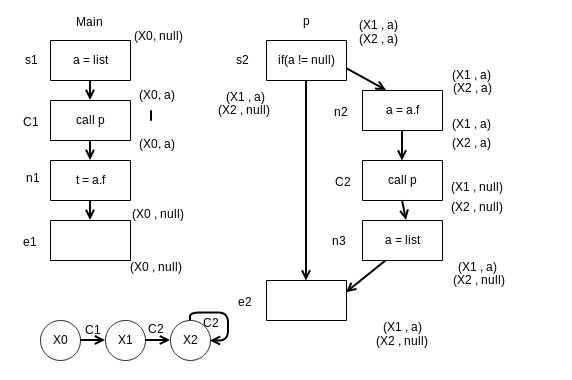
\includegraphics[width=7cm]{Figures/interproc_example.png}
\end{center}
\caption{Example for inter-procedural heap liveness}
\label{fig:extreme}
\end{figure}
	
	In the example the 2 contexts $X_1$ and $X_2$ are stored for the recursive procedure $p$.Value based contexts are used as a cache table for distinct call sites apart from terminating analysis of recursive procedures.
	
	

  \end{frame}
  
  \begin{frame}
  \frametitle{Analysis for concurrent programs}
  
  \begin{itemize}
  	\item Using the technique mentioned in the paper Dataflow Analysis for Datarace-Free Programs.
  	\item Produces an analysis for concurrent programs, given a sequential data-flow analysis
  	\item Criteria to apply this : The program should be free of data races. Data flow facts should be dependent on the contents of the memory access path.
  \end{itemize}
  
  \end{frame}
  
\begin{frame}
\frametitle{Analysis for concurrent programs}
Main challenge $\rightarrow$ converting the analysis for sequential programs to concurrent programs. How to propagate data-flow values to handle all possible thread execution orders?

\vspace{\baselineskip}
Synchronization structure of the program is made use of to propagate data-flow values

\vspace{\baselineskip}
The insight is that data-flow values are only propagated between threads at the lock and unlock points in threads. The relevant statements would usually be present inside the critical section.

\end{frame}  
  
  \begin{frame}
  \frametitle{Memory Model}
	\begin{itemize}
		\item Specifies the interactions of threads with memory and its shared use.
		\item Constraints on data access  
		\item Conditions of how data written by one thread is accessible to other threads
	\end{itemize}
	%Based on happens before-relation between two events. 
	Happens-Before Order: Statement  a happens before statement b if one of the following hold
	\begin{itemize}
		\item a appears before b in the program order
		\item b synchronizes-with a
		\item b can be reached transitively using happens-before relation from a.
	\end{itemize} 

  \end{frame}
  
\begin{frame}
\frametitle{Memory Model}

\begin{figure}
	\centering
	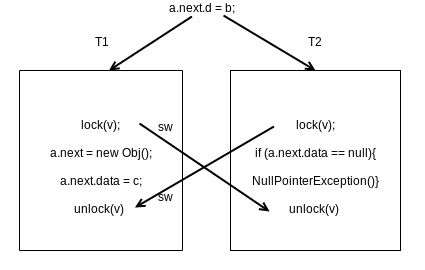
\includegraphics[width=0.6\textwidth]{Figures/sync_threads.png}
	\caption{Happens Before memory model with thread synchronization}
	\label{fig:happensbefore1}
	
	The \emph{NullPointerException} in $T_2$ cannot be raised because of the synchronizes-with relation between the lock and unlock statement. 
	
\end{figure}

\end{frame}

\begin{frame}
\frametitle{Memory Model}
\begin{figure}[b]
	\centering
	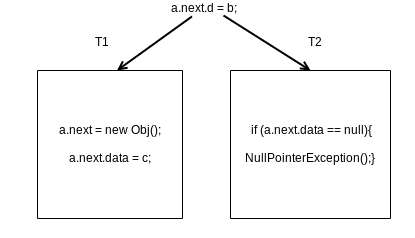
\includegraphics[width=0.5\textwidth]{Figures/sync_no_lock.png}
	\caption{Happens Before memory model without thread synchronization}
	\label{fig:happensbefore2}
\end{figure}

 	There is no synchronization relation between any statement across $T_1$ and $T_2$. There is no happens before order defined for statements across $T_1$ and $T_2$. So, NullPointerException() can be raised.
	
\end{frame}

\begin{frame}
\frametitle{Concurrent Null-Pointer Analysis}
	\begin{figure}
	\centering
	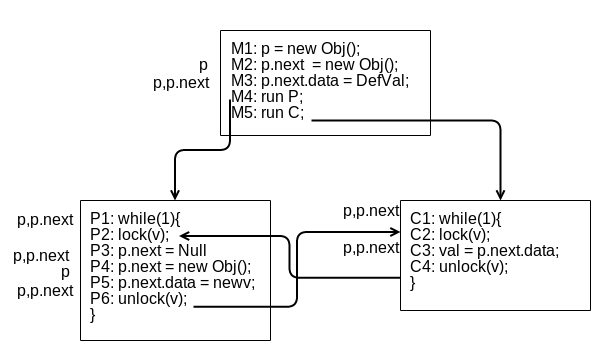
\includegraphics[width=0.75\textwidth]{Figures/concurrent_analysis.png}
	\caption{Heap Access path based null pointer analysis}
	\label{fig:nullpointeranalysis}
	\end{figure}
	
	\begin{itemize}
		\item Construction of sync-cfg by adding synchronization edges.
		\item Approximation of concurrent analysis to sequential analysis. Imprecise data flow values are obtained only at irrelevant statements.
	\end{itemize}
	 	
\end{frame}

\begin{frame}
\frametitle{Concurrent Null-Pointer Analysis}
	\begin{figure}
		\centering
		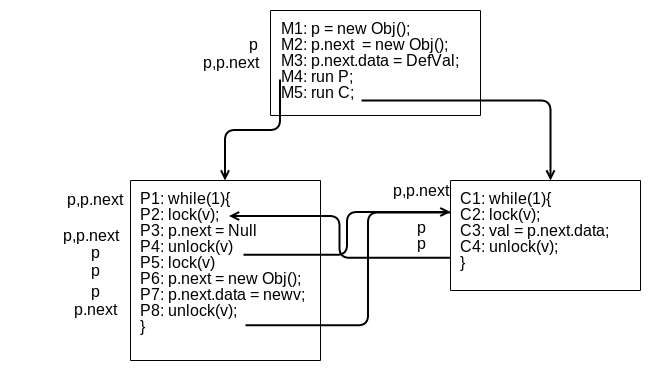
\includegraphics[width=0.75\textwidth]{Figures/concurrent_analysis_2.png}
		\caption{Heap Access path based null pointer analysis}
		\label{fig:nullpointeranalysis}
	\end{figure}
	
	Only $p$ is not-null at the statement C3, because of merging of values from P4 and P8.
	
\end{frame}

\begin{frame}
	\frametitle{Concurrent Heap Liveness Analysis}
	\begin{figure}
		\centering
		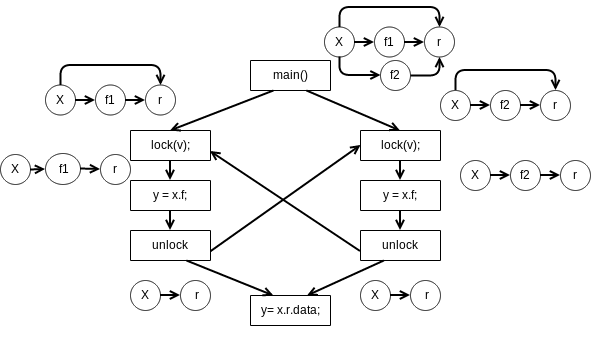
\includegraphics[width=0.7\textwidth]{Figures/concurrent_analysis_3.png}
		\caption{Concurrent Heap Liveness Analysis }
		\label{fig:nullpointeranalysis}
	\end{figure}
	The analysis is guaranteed to return correct data flow values at relevant program statements.
	 
\end{frame}

\begin{frame}
	\frametitle{Sync-cfg for Concurrent Heap Liveness}
	\begin{figure}
		\centering
		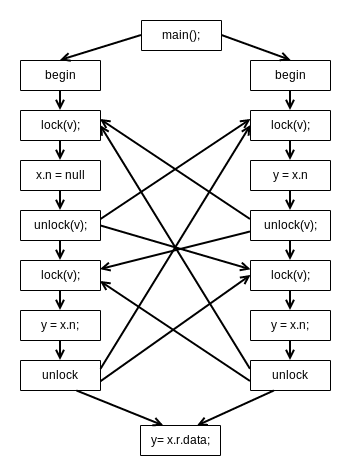
\includegraphics[width=0.5\textwidth]{Figures/hra_live_concurrent.png}
		\caption{Concurrent Heap liveness analysis input}
		\label{fig:nullpointeranalysis}
	\end{figure}
	
\end{frame}

\begin{frame}
	\frametitle{Example for concurrent heap liveness analysis}
	\begin{figure}
		\centering
		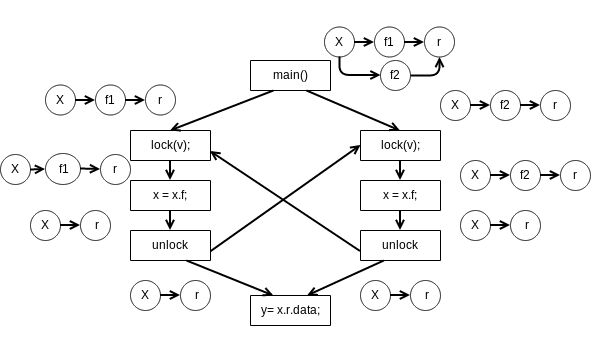
\includegraphics[width=0.8\textwidth]{Figures/conc_analysis_itr1.png}
		\caption{Concurrent Heap liveness analysis iteration 1}
		\label{fig:nullpointeranalysis}
	\end{figure}
\end{frame}

\begin{frame}
	\frametitle{Example for concurrent heap liveness analysis}
	\begin{figure}
		\centering
		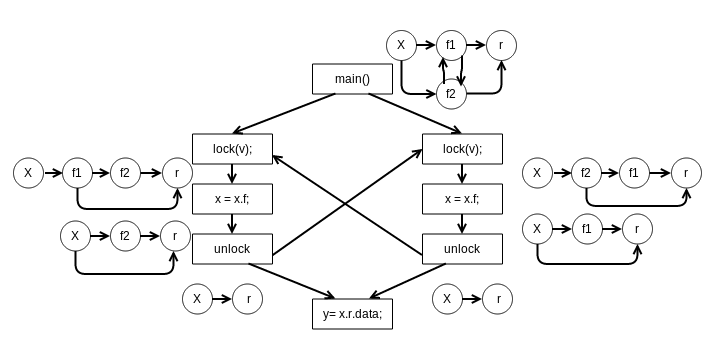
\includegraphics[width=0.8\textwidth]{Figures/conc_analysis_itr2.png}
		\caption{Concurrent Heap liveness analysis iteration 2}
		\label{fig:nullpointeranalysis}
	\end{figure}
\end{frame}

\begin{frame}
	\frametitle{Example for concurrent heap liveness analysis}
	\begin{figure}
		\centering
		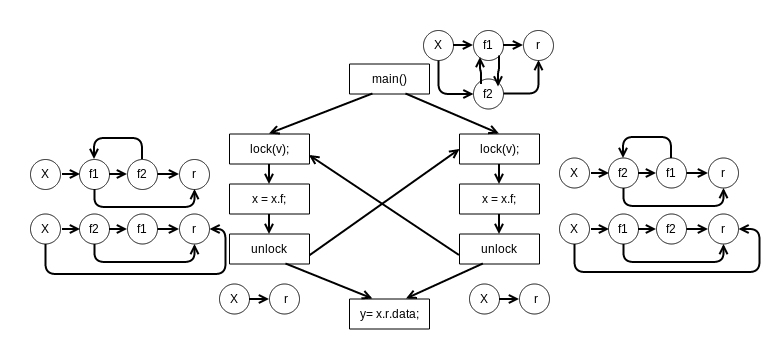
\includegraphics[width=0.8\textwidth]{Figures/conc_analysis_itr3.png}
		\caption{Concurrent Heap liveness analysis iteration 3}
		\label{fig:nullpointeranalysis}
	\end{figure}
\end{frame}

\begin{frame}
	\frametitle{Example for concurrent heap liveness analysis}
	\begin{figure}
		\centering
		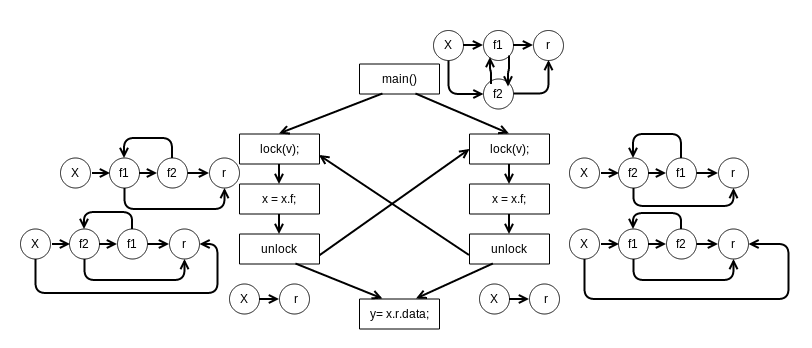
\includegraphics[width=0.8\textwidth]{Figures/conc_analysis_itr4.png}
		\caption{Concurrent Heap liveness analysis iteration 4}
		\label{fig:nullpointeranalysis}
	\end{figure}
\end{frame}


\begin{frame}
	\frametitle{Example for concurrent heap liveness analysis}
	Example of the same program without synchronization edges.
	\begin{figure}
		\centering
		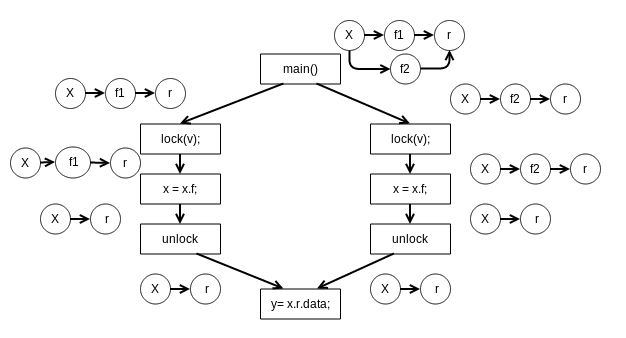
\includegraphics[width=0.8\textwidth]{Figures/conc_analysis_incorrect.png}
		\caption{Concurrent Heap liveness analysis without synchronization edges}
		\label{fig:nullpointeranalysis}
	\end{figure}
	An analysis without adding synchronization edges provides better results in this example. This highlights that there are certain problems with this analysis technique
\end{frame}

\begin{frame}
	\frametitle{Problems with the analysis technique}
	\begin{itemize}
		\item Propagation of
		data flow values across inter-thread edges  is treated same as along intra-thread edges.
		\item At program point containing the main statement, the possible live links can be be \emph{x.f1.f2.r} or \emph{x.f2.f1.r}.
		\item  Final data flow value  obtained after analysis includes imprecise access links \emph{x.f1.r}, \emph{x.f2.r} , \emph {x.\{f2.f1\}\textsuperscript{+}.r}, \emph{x.\{f1.f2\}\textsuperscript{+}.r} 
		
	\end{itemize}
\end{frame}

\begin{frame}
	\frametitle{Problems with the analysis technique}
	\begin{itemize}
		\item No bound on the number of transitions from node $f_1$ to $f_2$ and from $f_2$ to $f_1$ in the access graph.
		\item Thread synchronization edges introduce loops in the program graph
		\item Cause of imprecise data flow values is due to taking into account execution of critical sections more than once
	\end{itemize}
\end{frame}

\begin{frame}
	\frametitle{Problems with the analysis technique}
	Execution of multi-threaded programs
	\begin{itemize}
		\item Interleaving of statements of the multiple threads
		\item Addition of synchronization edges leads to formation of loop in the control flow graph
		\item Data flow value is transferred to every critical section multiple times
		\item Thus there is a need to identify the critical sections that only execute once
	\end{itemize}
\end{frame}

\begin{frame}
	\frametitle{Analysis of Critical Section Execution}
	Intra-thread Analysis to identify if critical section is executed once. 
	\begin{itemize}
		\item If there is no loop within and across a critical section, it can only be executed once.
		\item If a loop is present within a critical section, even then the critical section can be executed only once.
		\item It a loop is present across a critical section in a thread, then the critical section can be executed zero or more number of times.
	\end{itemize}
\end{frame}

\begin{frame}
	\frametitle{Adding Thread Info in Access Graphs}
	Once we know about the number of executions of each critical section there is a need to:  
	\begin{itemize}
		\item Need to figure out how to store the thread switchings in an access graph
		\item Store thread id corresponding to every edge in the access graph
		\item Identify which paths are possible with respect to the execution semantics.
		\item For example paths with multiple thread switches into a critical section can't be allowed.  
	\end{itemize}
\end{frame}


\begin{frame}
	\frametitle{Tools to Use}
	\begin{itemize}
		\item \emph{SOOT}: Java Byte Code Optimization Framework. Can implement precise intra-procedural analysis. SPARK engine provided call graph.
		\item \emph{VASCO}: Framework for carrying out precise inter-procedural analysis. Returns a better call graph as compared to SPARK.
		\item \emph{CombinedUnitGraph}: Generation of sync-cfg for programs containing upto 2 threads. Need to extend it to $n$ threads.
	\end{itemize}
\end{frame}

\begin{frame}

\Huge Thank You

\end{frame}
\end{document}